\section*{Espacio Cociente}

\begin{proposition}
    Sean \(X\) espacio topológico, \(Y\) un conjunto y \(\overset{\twoheadrightarrow}{\pi}:X\to Y\). La colección \(\tau_\pi = \{V\subset Y: \pi^{-1}(V)^\ab\subset X\}\) es una topología sobre \(Y\) a la que llamamos \emph{topología cociente}. 
\end{proposition}
\begin{definition}
    \(\overset{\twoheadrightarrow}{\pi}: X\to Y\) es una \emph{función cociente} si \(Y\) tiene la topología cociente definida por \(\pi\). 
\end{definition}
\begin{proposition}
    Si \(\pi\) es función cociente, entonces \(\tau_\pi\) es la topología más fina en \(Y\) tal que \(\pi\) es continua. 
\end{proposition}
\begin{proposition}
    Sean \(\pi\) función cociente y \(Z\) espacio topológico. Entonces \(f:Y\to Z \) es continua sii \(g\circ \pi: X\to Z\) es continua. 
\end{proposition}
\begin{proposition}
    Sea \(\overset{\twoheadrightarrow}{\pi}:X\to Y\) función continua entre espacios topológicos. Si \(\pi\) es abierta, entonces \(\tau_Y = \tau_\pi\).  
\end{proposition}

\E

\hrule 
\begin{example}
    Sea \(\mathbb{S}^1= \{(x,y)\in \R^2: x^2+y^2=1\}\) y \(\pi: [0,2\pi]\ni t \mapsto (\cos(t),\sin(t)) \in \mathbb{S}^1\).
\end{example}
\hrule 

\E
\newcommand{\D}{\mathcal{D}}
\newcommand{\A}{\mathcal{A}}

\begin{proposition}
    Sean \(X\) un espacio topológico y \(\D = \{A_i\subset X\}\) tal que \(A_i\cap A_j = \emptyset \) y \(\bigcup A_i = X\). Considere 
    \[\tau_\D = \left\{\A\subset \D: \left(\bigcup \{A : A\in \A\}\right)^\ab\subset X \right\}\]
    El conjunto \(\tau_\D \) es una topología en \(\D\) y \(\D\) es una descomposición de \(X\). Si \(x\in X\) entonces \(\exists !P_x \in \D \) tal que \(x\in P_x\). La función \(P_x: X\to \D\) es llamada \emph{función descomposición}. 
\end{proposition}
\begin{proposition}
    Toda descomposición \(P_x:X\to \D\) es una función cociente. 
\end{proposition}
\begin{proposition}
    Si \(\pi\) función cociente, entonces \(\exists P_x:X\to \D\) y un homeomorfismo \(f:Y\to \D\) tales que \(f\circ \pi = P\). 
\end{proposition}
\begin{definition}
    Sea \(X /\hspace{-0.1cm} \sim\) una relación de equivalencia. La descomposición \(\D\) formada por las clases de equivalencia de es llamada \emph{espacio de identificación} de \(X\) módulo \(\sim\). 
\end{definition}

\E

\hrule
\begin{example}
    Como vimos \(\mathbb{S}^1\) es un cociente del intérvalo \([0,2\pi]\). Aquí \(\D = \{\{x\}: x\in (0,2\pi)\}\cup \{\{0,2\pi\}\}\), donde \(x\sim y\) si \(x-y = 2k\pi\) con \(k\in \mathbb{Z}\). 
    \begin{figure}[!h]
    \centering
    % Primera subfigura: Intervalo [a, b]
    \begin{subfigure}{0.4\textwidth}
        \centering
        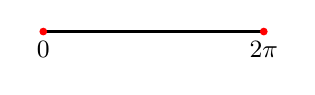
\begin{tikzpicture}[scale = 0.7]
            \draw[thick] (-2,0) -- (2,0);
            \fill[red] (-2,0) circle (2pt);
            \fill[red] (2,0) circle (2pt);
            \node[below] at (-2,0) {\small $0$};
            \node[below] at (2,0) {\small $2\pi$};
        \end{tikzpicture}
    \end{subfigure}
    \begin{subfigure}{0.4\textwidth}
        \centering
        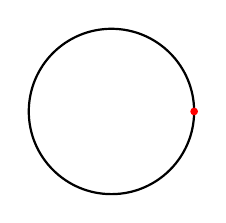
\begin{tikzpicture}[scale=0.7]
            \draw[thick] (-0.5,0) circle (1.5);
            \fill[red] (1,0) circle (2pt);
        \end{tikzpicture}
    \end{subfigure}
    
    \caption{\([0,2\pi]/\hspace{-0.1cm} \sim \)}
\end{figure}
\end{example}
\begin{example}
    Sea \(X = [0,2\pi]\times [0,2\pi]\) y \( (x_1,y_1)\sim (x_2,y_2)\) si \(x_1-x_2 = 2k\pi\) y \(y_1 = y_2\). El espacio \(X/\hspace{-0.1cm} \sim \ \ \cong \mathbb{S}^1\times [0,2\pi]\). 
\end{example}
\begin{example}
    Mismo \(X\) ahora con \( (x_1,y_1)\sim (x_2,y_2)\) si \(x_1-x_2 = 2k\pi\) y \(y_1 = y_2\) o si \(x_1=x_2\) y \(y_1-y_2 = 2k\pi\). En este caso \(X/\hspace{-0.1cm} \sim \ \ \cong \mathbb{S}^1\times \mathbb{S}^1\), el toro.  
\end{example}
\begin{figure}[!h]
    \centering
    % Primera subfigura: Identificación para el toro
    \begin{subfigure}{0.3\textwidth}
        \centering
        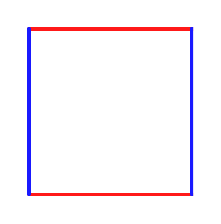
\begin{tikzpicture}[scale = 0.7]
            % Cuadrado base
            \shade[left color=red!90, right color=red!90, shading angle = 90] (0,0) rectangle (3,0.05);
            \shade[left color=red!90, right color=red!90, shading angle = 90] (0,3) rectangle (3,3.05);
            \shade[left color=blue!90, right color=blue!90, shading angle = 135] (0,0) rectangle (0.05,3.05);
            \shade[left color=blue!90, right color=blue!90, shading angle = 135] (2.95,0) rectangle (3,3.05);
       \end{tikzpicture}
        \caption{\(\mathbb{S}^1\times \mathbb{S}^1\)}
    \end{subfigure}
    \begin{subfigure}{0.3\textwidth}
        \centering
        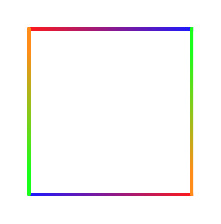
\begin{tikzpicture}[scale = 0.7]
            % Cuadrado base
            % \draw[thick, decorate, decoration = {linear color = red to blue}] (0,0) -- (0,3);
            \shade[left color=blue!90, right color=red!90, shading angle = 90] (0,0) rectangle (3,0.05);
            \shade[left color=red!90, right color=blue!90, shading angle = 90] (0,3) rectangle (3,3.05);
            \shade[left color=green!90, right color=orange!90, shading angle = 135] (0,0) rectangle (0.05,3.05);
            \shade[left color=orange!90, right color=green!90, shading angle = 135] (2.95,0) rectangle (3,3.05);
       \end{tikzpicture}
       \caption{Banda de Möbius}
    \end{subfigure}
\end{figure}
\begin{example}
    Mismo \(X\) con \( (x_1,y_1)\sim (x_2,y_2)\) si \(x_1-x_2 = 2k\pi\) y \(y_1 = y_2\) y \(y_1+y_2 = 2\pi\).  En este caso \(X/\hspace{-0.1cm} \sim \) es la banda de Möbius.  
\end{example}
\hrule 